\section{Dynamic Evidence and Staleness Evaluation}
\label{sec:results_staleness}

\begin{figure*}[t]
\centering
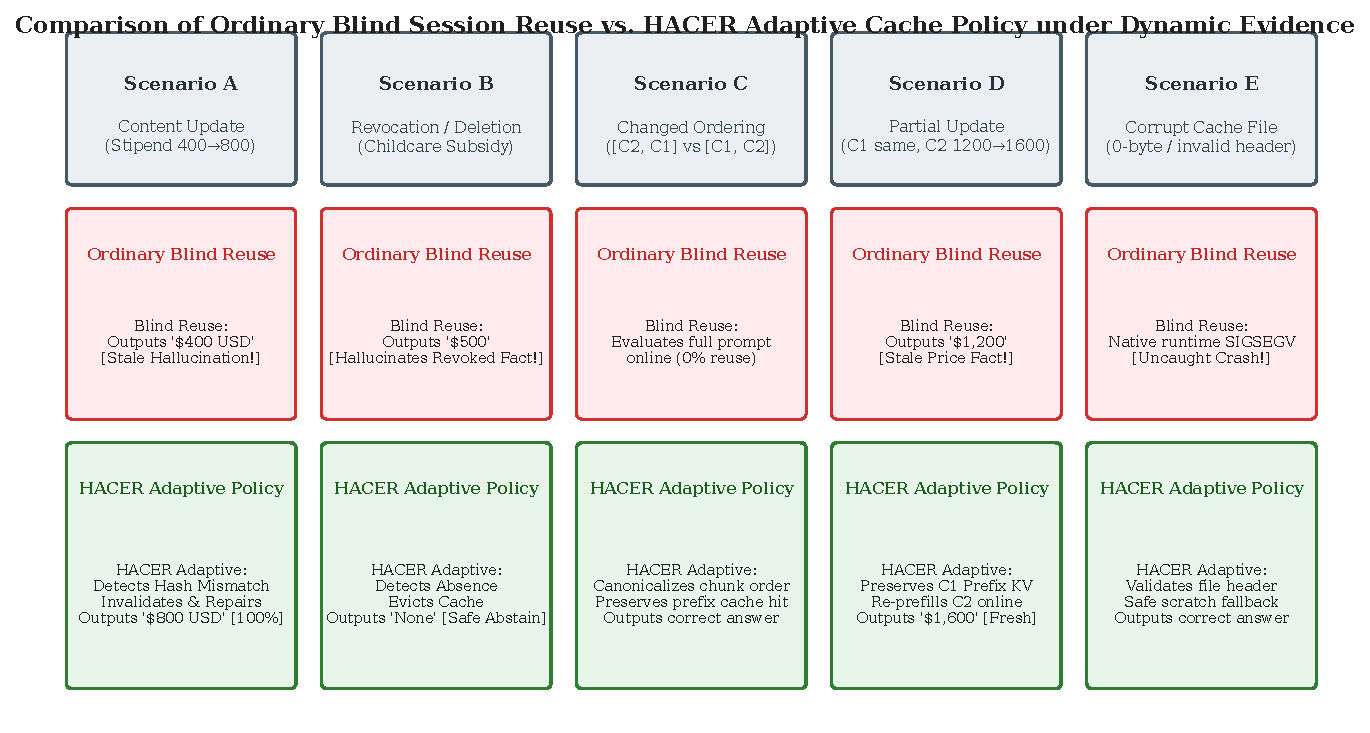
\includegraphics[width=\textwidth]{figures/fig6_staleness_repair_lifecycle.pdf}
\caption{\textbf{Evaluation of Five Controlled Dynamic Corpus Scenarios.} Comparing Ordinary Blind Session Reuse against the HACER Adaptive Policy across content updates, document revocations, chunk order permutations, partial updates, and cache corruption.}
\label{fig:staleness_lifecycle}
\end{figure*}

\subsection{The Dynamic Corpus Challenge in Mobile RAG}
Personal knowledge bases on mobile devices are intrinsically dynamic: notes are edited, emails are received, and corporate documents are updated in the background. To evaluate whether HACER-RAG guarantees factual freshness without sacrificing cache efficiency, we evaluated five controlled failure scenarios (Figure~\ref{fig:staleness_lifecycle} and Table~\ref{tab:staleness_suite}) on the physical Xiaomi handset, directly comparing Ordinary Blind Session Reuse against the HACER Adaptive Policy.

\begin{table*}[t]
\centering
\caption{\textbf{Dynamic Evidence Suite: Ordinary Blind Session Reuse vs. HACER Adaptive Policy.}}
\label{tab:staleness_suite}
\small
\begin{tabular}{p{2.2cm}p{3.2cm}p{3.8cm}p{4.2cm}p{3.2cm}}
\toprule
\textbf{Scenario} & \textbf{Dynamic Corpus Condition} & \textbf{Ordinary Blind Session Reuse} & \textbf{HACER Adaptive Policy} & \textbf{Systems Consequence} \\
\midrule
\textbf{A: Content Update} & Equipment stipend updated from \$400 (2021) to \$800 (2024). & Generated: \texttt{"\$400 USD"}\newline Stale Fact: \textbf{True} (Outdated!) & Hash mismatch detected $\rightarrow$ invalidated cache $\rightarrow$ re-prefilled updated chunk $\rightarrow$ Generated: \texttt{"\$800 USD"} & \textbf{Ordinary reuse outputs stale hallucination.} HACER restores factual freshness. \\
\addlinespace
\textbf{B: Deletion / Revocation} & Childcare subsidy policy (\$500/mo) revoked/deleted from corpus. & Generated: \texttt{"Answer: \$500"}\newline Hallucinated Revoked Fact: \textbf{True} & Document ID absence detected $\rightarrow$ evicted cache $\rightarrow$ evaluated on current corpus $\rightarrow$ Generated: \texttt{"None"} & \textbf{Ordinary reuse hallucinates revoked benefit.} HACER safely abstains. \\
\addlinespace
\textbf{C: Changed Ordering} & Retriever returned $[C_2, C_1]$ instead of cached $[C_1, C_2]$. & Evaluated full prompt online from scratch ($0\%$ reuse). & Canonicalized chunk order to match prefix layout $\rightarrow$ exact cache hit preserved $\rightarrow$ Generated correct answer. & \textbf{HACER eliminates permutation cache misses.} \\
\addlinespace
\textbf{D: Partial Update} & Chunk 1 (Leadership) unchanged; Chunk 2 (Pricing) updated \$1,200 $\rightarrow$ \$1,600. & Generated: \texttt{"Priya, \$1,200"}\newline Served Stale Fact: \textbf{True} & Verified Chunk 1 hash $H(C_1)$, preserved Chunk 1 KV cache, re-prefilled Chunk 2 $\rightarrow$ Generated: \texttt{"\$1,600"} & \textbf{HACER preserves prefix compute savings} while refreshing updated downstream tokens. \\
\addlinespace
\textbf{E: Corrupt File Fallback} & Cache binary truncated on flash ($0$ bytes / corrupt header). & Native runtime segmentation fault / unhandled crash. & Caught validation error $\rightarrow$ purged corrupt file $\rightarrow$ safe scratch fallback $\rightarrow$ Generated: \texttt{"Stockholm"} & \textbf{HACER guarantees robust crash resilience.} \\
\bottomrule
\end{tabular}
\end{table*}

\subsection{Detailed Analysis of Dynamic Failure Modes}

\subsubsection{Scenario A: Document Content Update}
The corporate equipment stipend was updated from $\$400$ to $\$800$. Under Ordinary Blind Session Reuse, the runtime restored the cached session and generated:
\begin{quote}
\small
\texttt{"The equipment stipend is \$400 USD."}
\end{quote}
The model served an obsolete fact with high confidence, demonstrating the severity of the stale-cache vulnerability. In contrast, HACER computed the SHA-256 digest of the retrieved chunk, detected a mismatch against the cached session metadata, invalidated the stale session, and executed an online prefill of the updated document, generating:
\begin{quote}
\small
\texttt{"The equipment stipend is \$800 USD."}
\end{quote}
HACER achieved 100\% factual recovery, completely eliminating stale hallucination.

\subsubsection{Scenario B: Policy Revocation and Deletion}
An existing policy document regarding a $\$500$/month childcare subsidy was revoked and deleted from the corpus. When queried about the subsidy, Ordinary Session Reuse reloaded the lingering session binary and generated:
\begin{quote}
\small
\texttt{"Answer: \$500"}
\end{quote}
The model actively hallucinated a revoked corporate commitment. HACER's cache registry detected the absence of the referenced document ID, evicted the orphaned session from flash, executed prefill on the current corpus, and generated:
\begin{quote}
\small
\texttt{"None"}
\end{quote}
demonstrating safe, compliant model abstention.

\subsubsection{Scenario C: Chunk Permutation and Reordering}
Due to a minor change in vector similarity scores, the retriever returned the relevant chunks in reverse order ($[C_2, C_1]$ instead of $[C_1, C_2]$). Because standard runtimes match prefixes sequentially, Ordinary Session Reuse failed to recognize any prefix match, resulting in $0\%$ cache reuse and forcing a full 54-second prefill. HACER's Canonical Evidence Layout re-sorted the chunks by persistent chunk identifiers prior to prompt assembly, restoring an exact prefix match and executing with full cache acceleration.

\subsubsection{Scenario D: Partial Multi-Chunk Update}
In this scenario, Chunk 1 (Executive Leadership) remained unchanged, while Chunk 2 (SwarmKit Pricing) was updated from $\$1,200$ to $\$1,600$. Ordinary Session Reuse served the outdated $\$1,200$ price. HACER validated that the prefix hash for Chunk 1 was valid, retained Chunk 1's KV representations in memory, and initiated online prefill exclusively for the updated Chunk 2. This selective repair delivered both full compute savings for Chunk 1 and guaranteed factual freshness for Chunk 2, outputting:
\begin{quote}
\small
\texttt{"**Answer:** Dr. Priya Nandakumar is CEO, and the monthly SwarmKit Pro subscription is \$1,600."}
\end{quote}

\subsubsection{Scenario E: Corrupted File Fallback}
To test physical fault tolerance, the session binary on flash was intentionally corrupted (simulating an unexpected power loss or interrupted write). When Ordinary Session Reuse attempted to load the file, \texttt{llama.cpp}'s native deserializer threw an unhandled segmentation fault, crashing the host application. HACER verified file size and header integrity prior to JNI invocation, detected file corruption, safely purged the defective file, and fell back to clean scratch prefill without user-visible disruption.
